\subsection{UAP Algorithmus}

Unser Algorithmus für universelle adversarielle Perturbationen (UAP) basiert auf dem Ansatz von Moosavi-Dezfooli et al. \cite{moosavi-dezfooli_universal_2017}. Ziel ist es, eine Perturbation zu entwickeln, die auf neue Bilder übertragbar ist. Dies erreichen wir, indem wir iterativ durch eine Auswahl von Trainingsbildern gehen und den jeweils kürzesten Weg zur Entscheidungsgrenze jedes Bildes finden. Die dabei erzeugten Perturbationen werden summiert, um eine universelle Perturbation zu formen. 

\subsubsection{Loss-Funktion}
Das Optimierungsproblem wird bei unserer Umsetzung durch eine Loss-Funktion gelöst, welche die Norm der Perturbationsmatrix und die invertierte Binary Cross Entropy Funktion minimiert. Diese sieht wie folgt aus:

\begin{equation}
    L_{UAP} = \lambda_{norm} \cdot ||v + \Delta v||_p + \frac{1}{L_{BCE}(\hat{y}, \hat{y}_{adv}) + \epsilon}
\label{Loss}
\end{equation}

Wobei der hier verwendete BinaryCrossEntropy Loss kann wie folgt minimiert werden:

\begin{equation}
L_{BCE} = - (\hat{y} \cdot \log(\hat{y}_{adv}) + (1-\hat{y}) \cdot \log(1-\hat{y}_{adv}))
\label{eq:BCE}
\end{equation}

\begin{align*}
\text{Wobei:}&\\
L_{UAP}, &\text{ ist der gesamte Loss.} \\
L_{BCE}, &\text{ bezeichnet den Binary-Cross-Entropy Loss.} \\
\lambda_{norm}, &\text{ ist der Regularisierungsparameter.} \\
v, &\text{ ist die universelle Störung.} \\
\Delta v, &\text{ ist die Änderung der Störung.} \\
||v + \Delta v||_p, &\text{ repräsentiert die } L_p \text{-Norm der Perturbation } v + \Delta v. \\
\hat{y}, &\text{ ist die Vorhersage des Modells für das Originalbild.} \\
\hat{y}_{adv}, &\text{ ist die Vorhersage des Modells für das perturbierte Bild.} \\
\epsilon, &\text{ ist eine kleine positive Konstante für numerische Stabilität.}
\end{align*}

Da unser Algorithmus eine Batch Size von 1 erfordert und nach jeder Berechnung die Backpropagation durchführt, muss bei der Loss-Funktion kein Mittelwert berechnet werden. $\hat{y}$ sowie $\hat{y}_{adv}$ beziehen sich auf das aktuelle Bild im Algorithmus.

Für $\epsilon$ wird ein kleiner Wert wie $1^{-6}$ gewählt, der eine Division durch Null verhindert, wenn der Output unseres Modells sowohl mit als auch ohne Störung gleich ist. Dies ist vorallem bei der Berechnung der allerersten Perturbation ein Problem.

\newpage
\subsubsection{Technische Umsetzung}
Die technische Umsetzung des Prozesses zur Generierung der UAP-Bilder ist in der folgenden Grafik \ref{fig:05-uap_algorithm} dargestellt:

\begin{figure}[H]
    \centering
    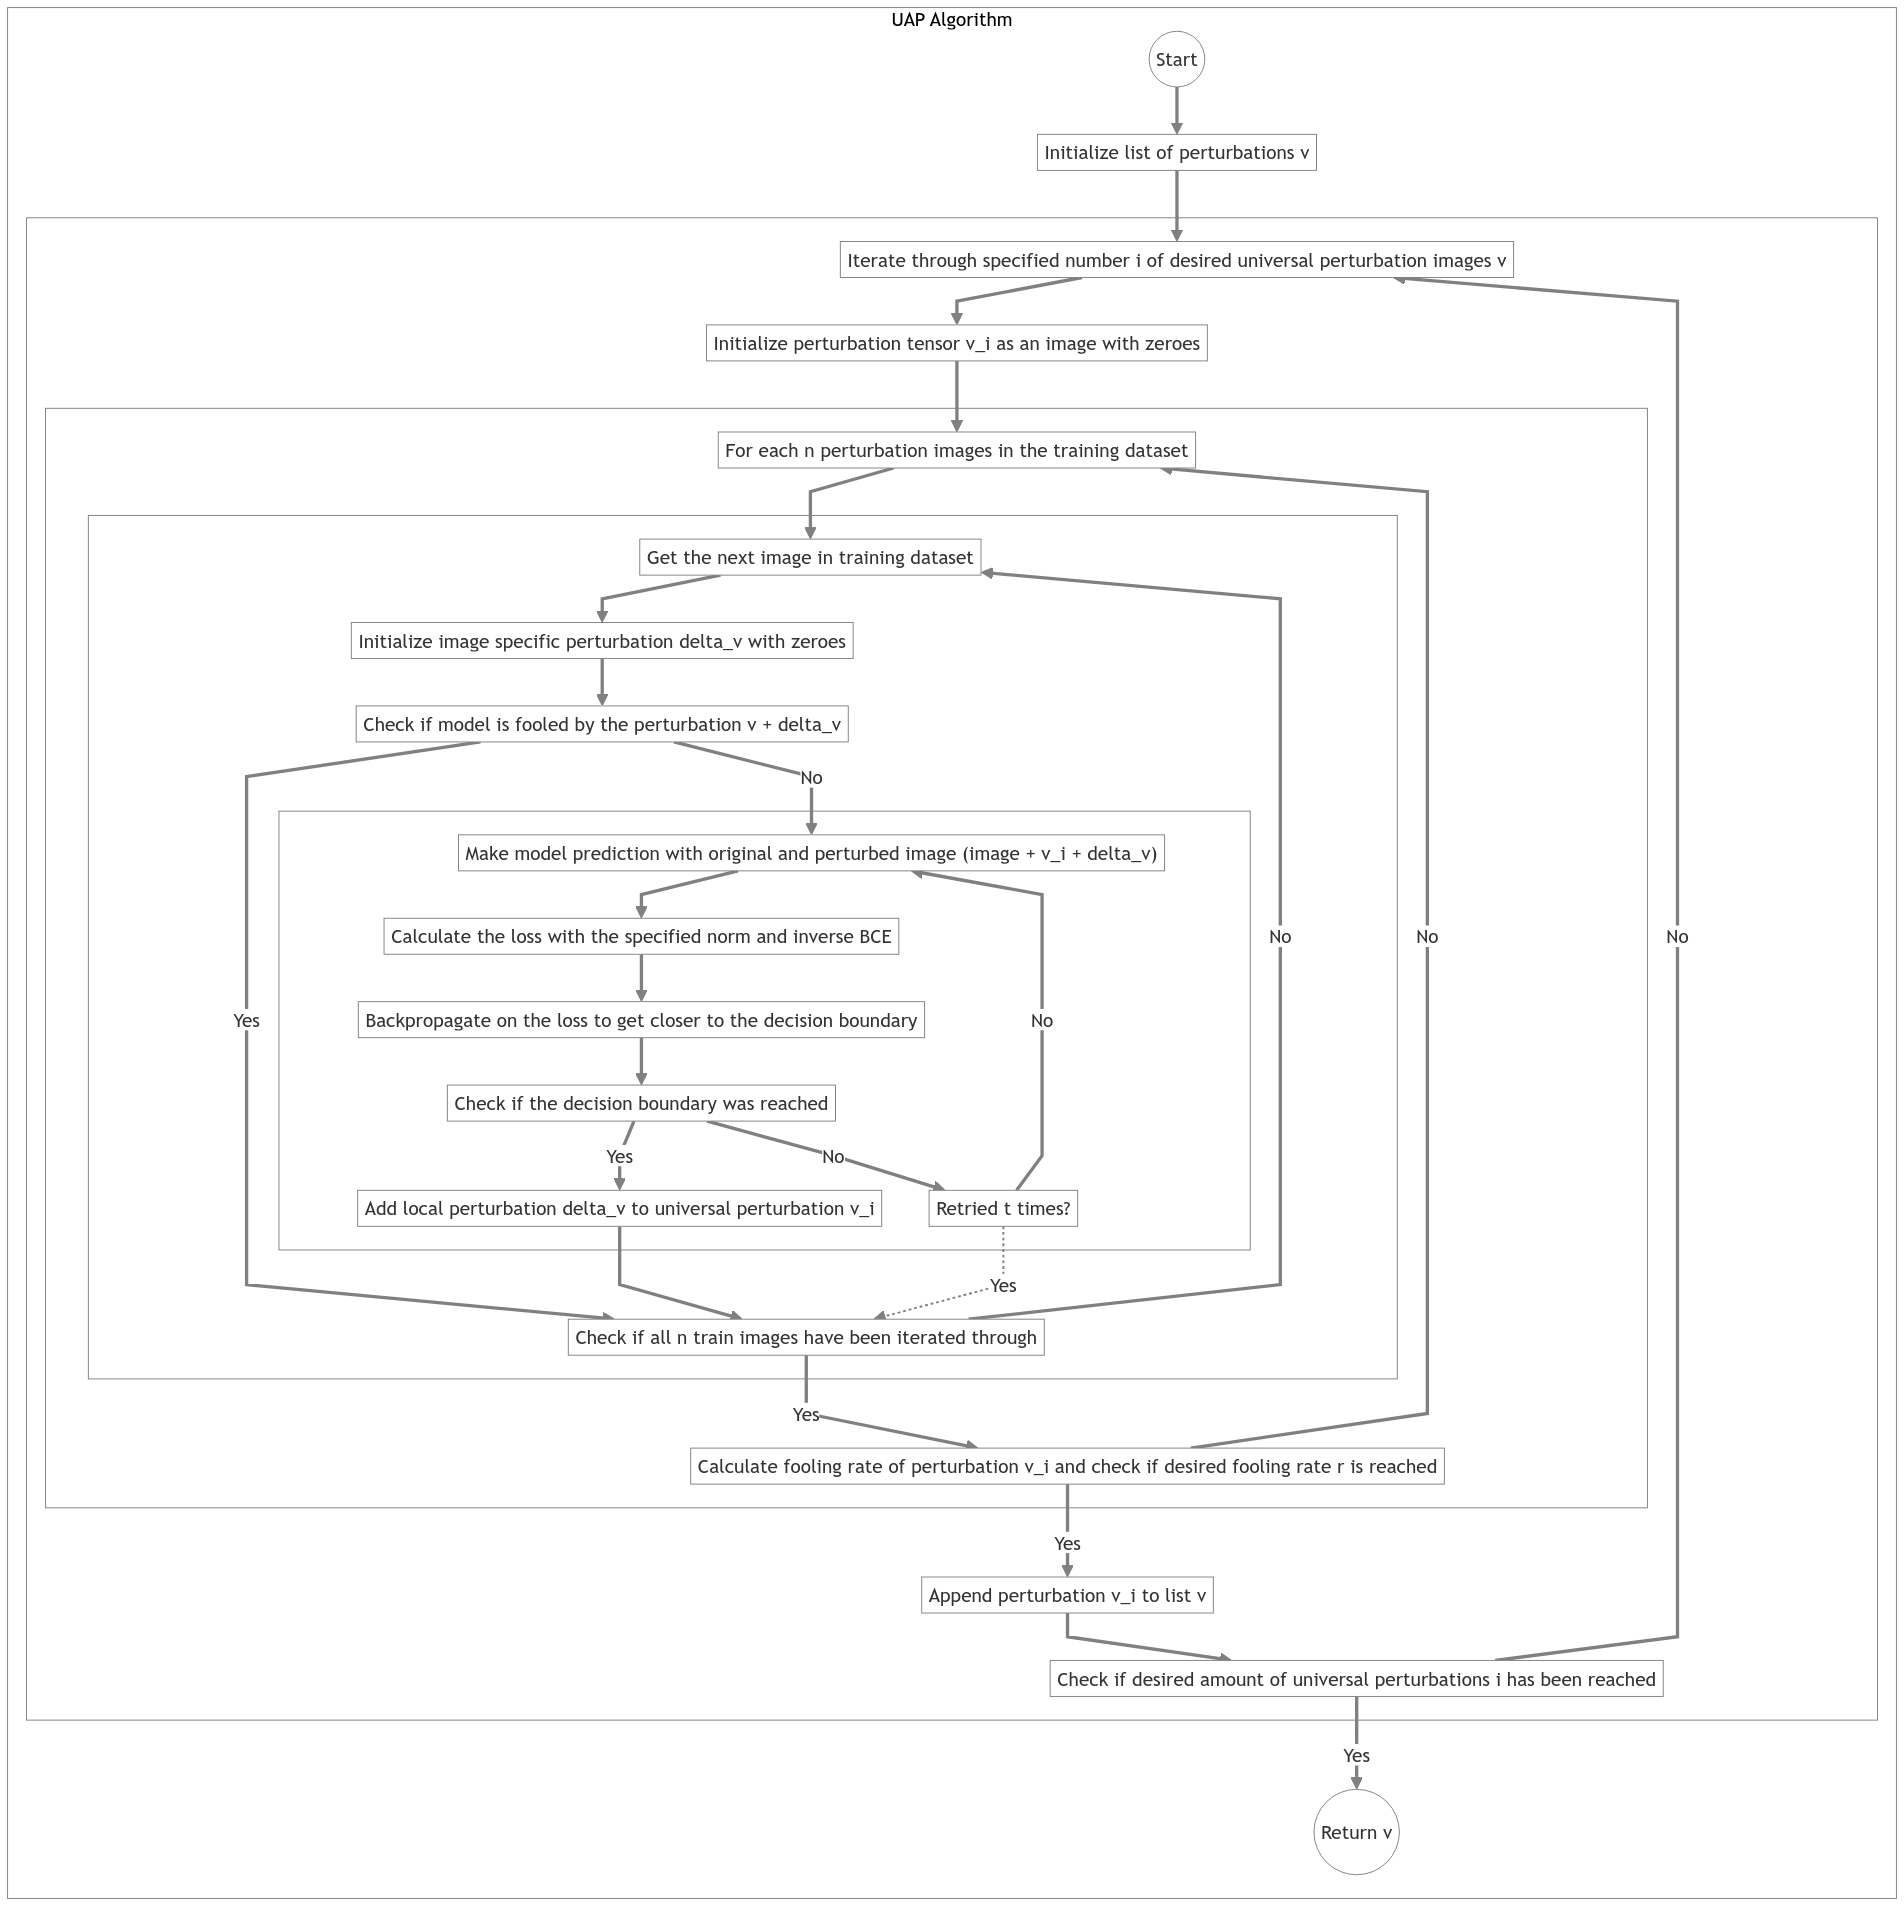
\includegraphics[width=14.5cm]{01-images/05-UAP_ALG}
    \caption{UAP Algorithmus}
    \label{fig:05-uap_algorithm}
\end{figure}


\text{Wobei man folgende Parameter selbst bestimmen muss:}
\begin{align*}
i, &\text{ ist die Anzahl Perturbationsbilder, welche generiert werden sollen.} \\
n, &\text{ ist die Anzahl Trainingsbilder, welche für die Generierung verwendet werden.} \\
t, &\text{ ist die Anzahl Versuche, eine bildlokale Perturbation zu finden}\\
r, &\text{ ist der prozentuelle Anteil von Trainingsbilder, welche durch die Perturbationen} \\ 
&\text{  getäuscht werden soll, damit die Perturbation } v_i \text{ gespeichert wird.} \\
p, &\text{ ist der Normparameter der } L_p \text{ Norm.}\\
\lambda_{norm}, &\text{ siehe Loss-Funktion.}\\
\epsilon, &\text{ siehe Loss-Funktion.}
\end{align*}